\chapter{Introduction}
\label{ch:introduction}

\def\figdir{chapters/ch01_introduction/figures}

%\epigraph{\textit{The easiest way to solve a problem is to deny it exists.}}{Isaac Asimov}

%\begin{quote} 
%	\begin{flushright}
%		\textit{The easiest way to solve a problem\\ is to deny it exists.}
%		
%		--- ~ Prof. Isaac Asimov
%	\end{flushright}
%\end{quote}

\section{Motivation}

\lettrine[lines=3,nindent=0em,loversize=0.1]{T}{he} global population is steady rising and migrating from rural areas to urban areas and results in a growing urbanization as urban for past two centuries. This result of a rapid rise in urban population and therefore in future the ecology of the urban system will become a primary concern. Furthermore, climate change, driven by human activity need to be reduces to mitigate the present detrimental climatology in urban areas. A lack thereof can not only have implication on the global climate but also the comfort and health of urban populace. 

Therefore, presently, there is an increasingly growing need to accurately predict the impact of the vegetation at scale of pedestrians. Vegetation provides natural cooling through shading and transpiration and is a primary solution to combat the growing urban heat island (UHI) and improve the thermal comfort  \citep{Gillner2015, Bowler2010, Loughner2012}. 

\begin{figure}[h]
	\centering
	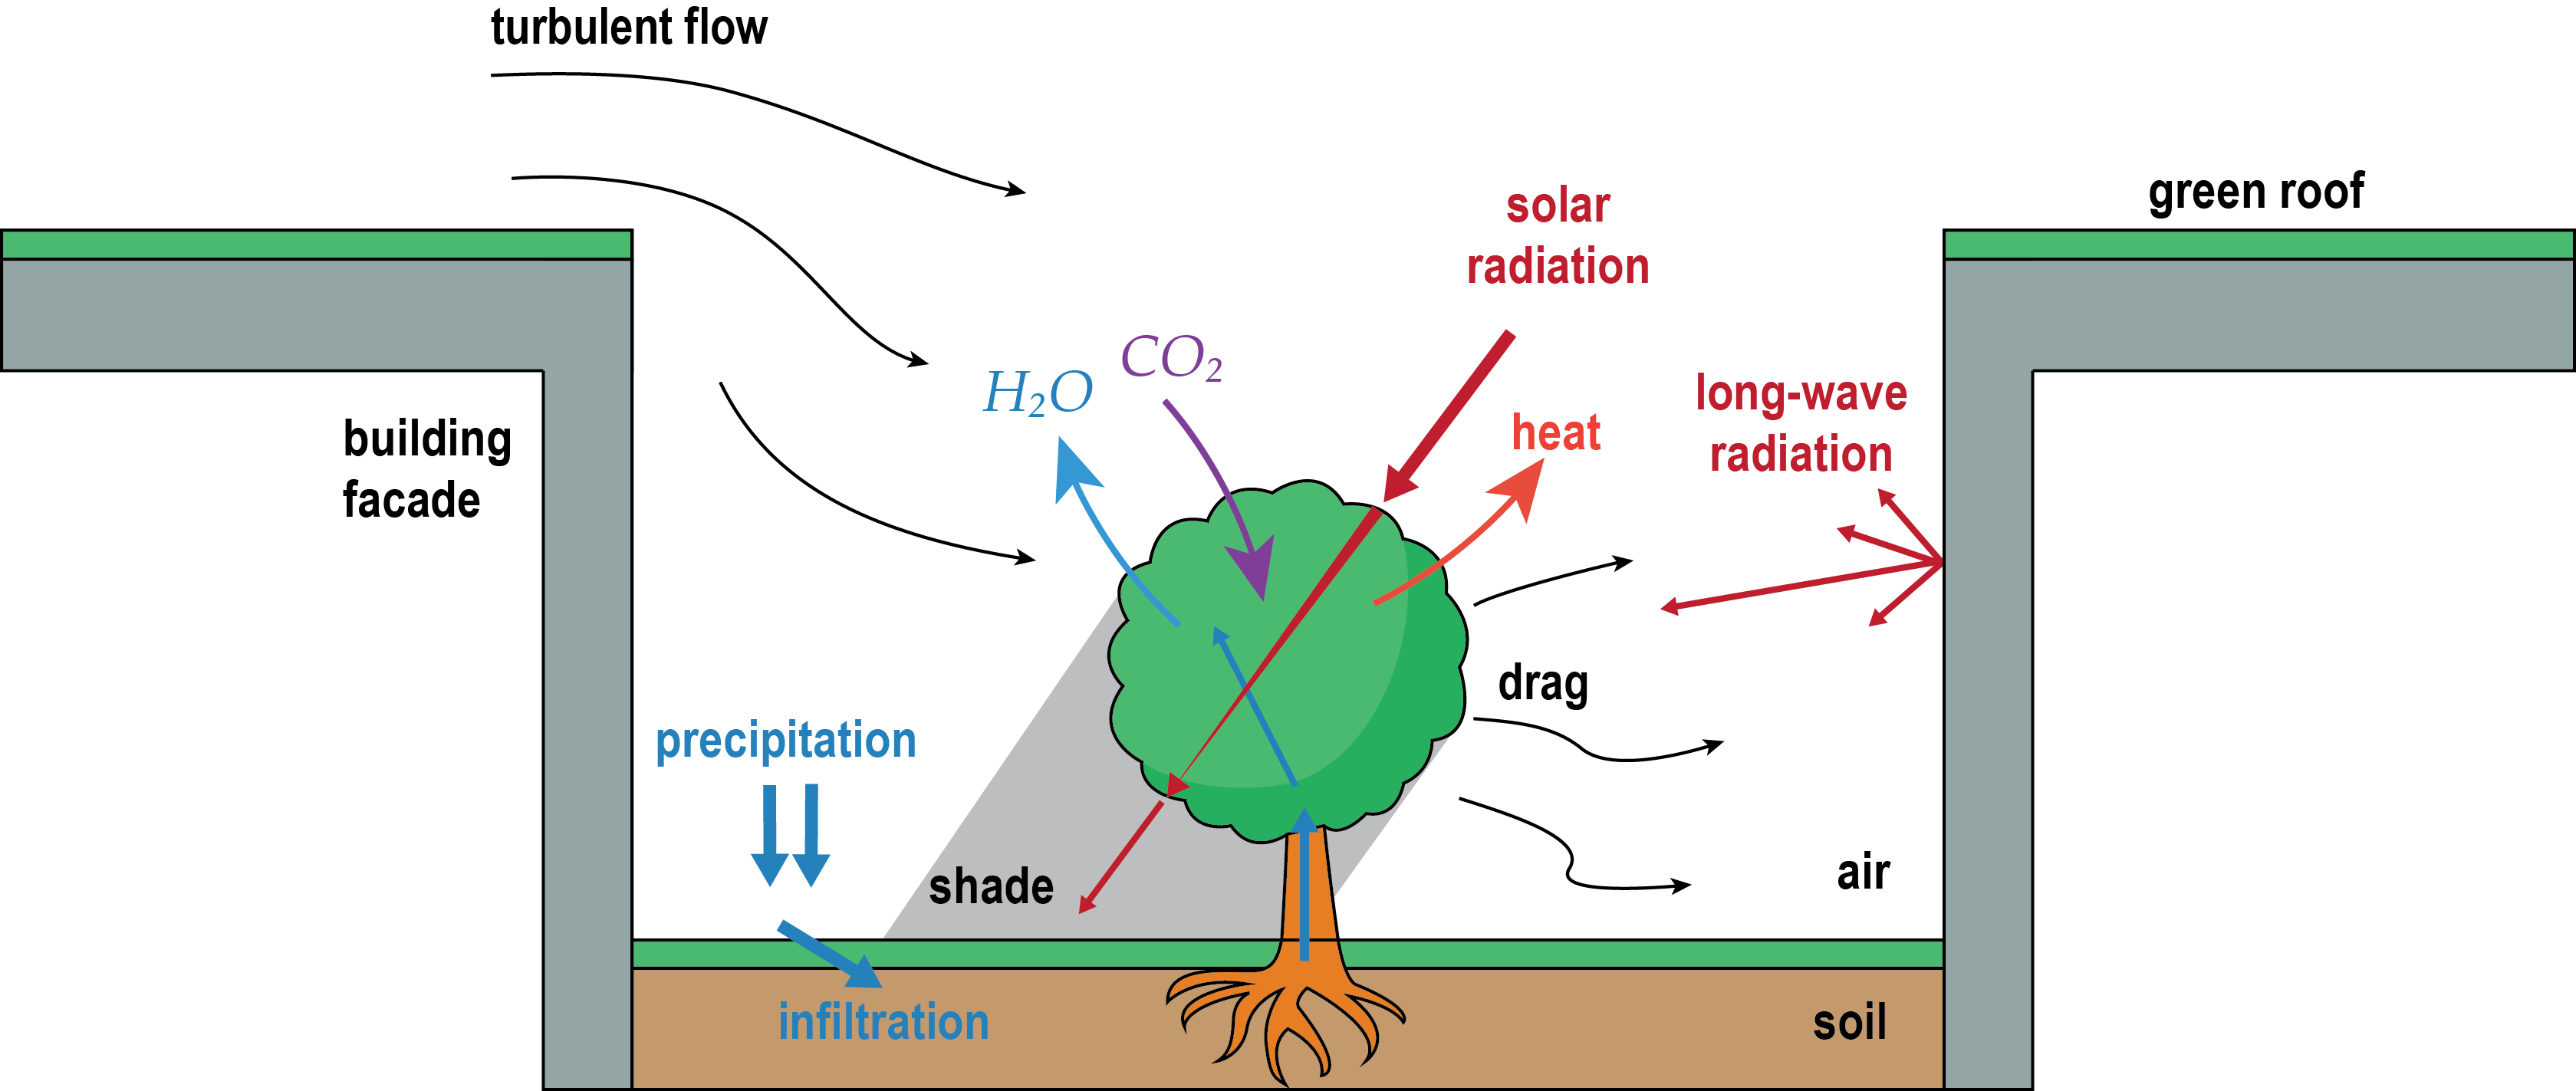
\includegraphics[width=\textwidth]{\figdir/streetcanyon_tree_part5.png}
	\caption{Interaction of urban vegetation with the urban microclimate.}
	\label{fig:vegetation_fluxes}
\end{figure}

The complexifiers which make in urban greening solutions is that cooling provided by vegetation is environmentally dependent. Figure \ref{fig:vegetation_fluxes} shows a schematic representation of the various fluxes exchanged between an urban tree and the environment. The figure shows the the various physical processes that vegetation is part of. The solar radiation is absorbed by plant foliage and drives the energy balance that controls the latent (i.e., due to transpiration of moisture), and sensible heat flux from the plant. Furthermore, the interception of solar radiation provides shading in the urban area. Vegetation also has an impact on the water cycle, where the moisture in the soil is transported into air through transpiration. Moreover, the plant transpiration is dependent on the water availability at the plant roots. %So, the transpiration driven cooling (i.e., transpirative cooling potential) of vegetation is environmentally dependent. 


Furthermore, high vegetation density can also have a negative impact on the ventilation characteristics in an urban microclimate. So, increasing the thermal comfort in urban area can be at the cost of air quality. Thus, there exists a need for a numerical prediction tool that can take into account of all these factors to provide an accurate assessments on the impact of vegetation in urban microclimate. 

\section{Objective and Methodology}

The goal of the thesis is to improve the assessment on the impact of vegetation on the urban microclimate. As vegetation is increasingly being sought after as a natural UHI mitigation strategy, accurate predictions are need to assess their effectiveness. More specifically, the objective of this thesis is as follows:
\begin{itemize}
	\item to assess the impact of vegetation on the microclimate.
	
	\item to quantify the natural cooling (i.e., transpirative cooling and shading) provided by vegetation in urban microclimate.
	
	\item to understand the influence of water stress on the natural cooling.
	
	\item to quantify the impact of vegetation on pedestrian thermal comfort. 
\end{itemize}

Experimental and numerical approaches are employed to assess the impact of vegetation on the microclimate. Wind tunnel experiments in an atmospheric boundary layer (ABL) are opted to understand the impact of vegetation on the airflow and the local microclimate, where small model trees and small natural trees are employed as scaled models. Measurement techniques such as particle image velocimetry (PIV) and drag force measurement are employed to quantify the modification of airflow due to vegetation. Measurement techniques such as infrared thermography, and hygrothermal sensor analysis are used to quantify the change in hygrothermal variables. A numerical asssessment on the impact of vegetation on urban microclimate is achieved by developing a vegetation model integrated into a computation fluid dynamics  (CFD) model. The numerical model simultaniously takes in account of the turbulence modification, radiation balance, heat and mass fluxes, and the sensitivity to soil moisture simultaneously. With this modeling technique, the cooling potential of vegetation is quantified along with the impact on thermal comfort for a pedestrian. 

\section{Outline of the thesis}

This thesis is divided into two parts: i) experimental studies (\cref{ch:paper2,ch:microclimatestudy}), and ii) numerical studies (\cref{ch:parametricstudy,ch:wtcfdcomparison,ch:numericalmethod,ch:impactofvegetation}) of the impact of vegetation on urban microclimate. The thesis is organized as follow:
\begin{itemize}
	\item \textit{Chapter 2}: The chapter addresses the state of the art providing an overview on the urban climate, the impact of vegetation on urban microclimate, experimental approaches for assessing the impact of vegetation, and numerical approaches for assessing the impact of vegetation in urban microclimate. The goal of the chapter is: i) to provide relevant researches that are present and are employed for determining the impact of vegetation in urban microclimate, ii) to provide a justification on the development of the numerical model that is presented in this thesis, and iii) to give the scope of the numerical model. 

	\item \textit{Chapter 3}: This chapter is the first part of the experimental studies, where the impact of vegetation on the airflow is investigated. The influence of vegetation on the airflow is studied in an atmospheric boundary layer (ABL) wind tunnel using model and small natural trees. In the study, the turbulent airflow behind the trees is studies using particle image velocimetry (PIV) measurement technique and is linked to the drag force measurements using a load cell. The chapter has been published as: Manickathan, L., Defraeye, T., Allegrini, J., Derome, D., \& Carmeliet, J. (2018). ``Comparative study of flow field and drag coefficient of model and small natural trees in a wind tunnel''. \textit{Urban Forestry \& Urban Greening}, 230–239. \url{http://doi.org/10.1016/j.ufug.2018.09.011}.
	%The study investigates the sheltering provided by small model trees and how it differs from that of small natural trees. Thereafter, the flow field and drag coefficient of model trees are compared to the ones of natural trees of similar size to determine whether model trees can be used to represent natural trees. 
	
	\item \textit{Chapter 4}: This chapter is the second part of the experimental studies, where the impact of vegetation on the microclimate is investigated. The influence of vegetation on the microclimate is studied in the wind tunnel using small plant: \textit{Buxus sempervirens}. In the study, the diurnal dynamics of the plant microclimate of a \textit{Buxus sempervirens} is investigated using various high-resolution non-intrusive imaging techniques. The wake flow field is measured using stereoscopic particle image velocimetry (SPIV), the spatiotemporal leaf temperature history is obtained using infrared thermography, and the plant microstructure metrics such as plant porosity, leaf area density (LAD) is obtained through X-ray tomography. %The study helps us answers the following questions: What is the spatial and temporal variability of the plant cooling due to environmental conditions such as wind speed and solar radiation? What is the diurnal response of the plant? Moreover, the experiment provides a high-resolution dataset for future validation studies.
	
	\item \textit{Chapter 5}: This chapter is the first part of the numerical studies, where the impact of vegetation on the transpirative cooling potential is investigated. The influence of vegetation on the transpirative cooling is studied using a computation fluid dynamics (CFD) modeling approach, where vegetation is modeled as porous medium. In the chapter, a parametric study on the influence of environmental factors (i.e., wind speed, air temperature, relative humidity and solar radiation intensity) and tree properties (i.e., leaf size, stomatal resistance and leaf area density) on the transpirative cooling effect of trees is performed. Furthermore, the Universal Thermal Climate Index (UTCI) around the trees is evaluated to determine the impact of transpirative cooling on pedestrian thermal comfort. The chapter has been published as: Manickathan, L., Defraeye, T., Allegrini, J., Derome, D., \& Carmeliet, J. (2018). ``Parametric study of the influence of environmental factors and tree properties on the transpirative cooling effect of trees''. \textit{Agricultural and Forest Meteorology}, 248, 259–274. \url{http://doi.org/10.1016/j.agrformet.2017.10.014}.%It porous medium approach provides the necessary source terms for heat, mass, momentum, and radiative fluxes due to vegetation. 
	
	\item \textit{Chapter 6}: This chapter is focuses on comparing the developed numerical in \cref{ch:parametricstudy} with wind tunnel measurements of \cref{ch:microclimatestudy}. The goal of the chapter is to compare and determine the discrepancy of the numerical model in predicting the airflow and the transpiration cooling of vegetation. 
	
	\item \textit{Chapter 7}: This chapter the numerical model of assessing the impact of vegetation in urban microclimate is described. The \textit{air} domain solver, the \textit{solid} domain solver, and the \textit{radiation} model is described in detail. Furthermore, the chapter describes the coupling strategy employed to couple these three models which an overview of the coupling algorithm. The influence of water availability on transpiration rate is addressed using a modified stomatal model based on the soil-plant-atmosphere continuum (SPAC) model approach. 
	
	\item \textit{Chapter 8}: This chapter is the second part of the numerical studies, where the impact of vegetation on the urban microclimate is investigated using the numerical model described in \cref{ch:numericalmethod}. The impact of vegetation on the urban microclimate consists of modification to the urban turbulent airflow, addition of transpirative cooling in urban area, and the plant shading provided by the foliage. The influence of these phenomena is investigated together with the impact of pedestrian thermal comfort. 
	
	\item \textit{Chapter 9}: Finally, this chapter provides a conclusion and some of the main finding in the thesis. Furthermore, the chapter provides an overview to the contributions to the research field from the present thesis. An outlook and possible future research aspects is given thereafter.
	
\end{itemize}

